\documentclass[11pt]{article}

\usepackage{filecontents}
\usepackage{graphicx}
\graphicspath{{/Users/laci/Schule/Diplomarbeit_GitHub/LATEX_DOKU_DA/src}}
\usepackage{tabularx}
\usepackage{multirow}
\usepackage{xcolor}
\usepackage{caption}
\usepackage[autostyle]{csquotes}
\usepackage{circuitikz}
\usepackage{amsmath}
\usepackage{textgreek}
\usepackage{siunitx}
\usepackage[utf8]{inputenc}
\usepackage[ngerman]{babel}
\usepackage[margin=2.5cm]{geometry}
\usepackage[none]{hyphenat}
%==========================================================================
\usepackage{fancyhdr}
\pagestyle{fancy}
\fancyhead[L]{\MakeUppercase{Diplomarbeit 5BHEL 23/24}}
%\fancyhead[R]{\chead{
\includegraphics[width=\textwidth]{src/TGM.jpg}}}
\fancyfoot[L]{\small{Al-Maytah, Schweitzer, Szabo}}
\fancyfoot[C]{}
\fancyfoot[R]{\arabic{page}}

\usepackage[round, sort, authoryear]{natbib}
%\usepackage[nottoc]{tocbibind}
%==========================================================================
%==DOKUMENTBEGINN==========================================================

\begin{document}

%==========================================================================
%==TITELSEITE==============================================================

\begin{titlepage}
	
	\title{\textbf{\Huge{Diplomarbeit}}}
	\maketitle
	\thispagestyle{empty}

	\begin{center}

		\hfill \break
		\hfill \break
		\hfill \break
		\textbf{\Large{Gesamtprojekt}} \break
		\par
		\textbf{\LARGE{RoboGlove - Bionische Hand}}

		\hfill \break
		\hfill \break
		\hfill \break
		\hfill \break
		\hfill \break

		\begin{tabular}{p{10cm}p{1cm}l}
			3D-Druck, Mechanik und User-Interface-Programmierung \\
		\end{tabular}

		\begin{tabular}{p{3cm}p{2cm}l}
			Amir Al-Maytah & 5BHEL & Betreuer: Dipl.-Ing. Christoph Diemberger \\
		\end{tabular}

		\begin{tabular}{p{3.26cm}p{5cm}l}
			& Fachlehrer: Robert Offner 
		\end{tabular}

		\hfill \break

		\begin{tabular}{p{14cm}p{1cm}l}
			Mikrokontroller-Promgrammierung, Testmanagement und Gesamtintegration \\
		\end{tabular}

		\begin{tabular}{p{3cm}p{2cm}l}
			Fabian Schweitzer & 5BHEL & Betreuer: Dipl.-Ing. Christoph Diemberger \\
		\end{tabular}

		\begin{tabular}{p{3.26cm}p{5cm}l}
			& Fachlehrer: Robert Offner 
		\end{tabular}

		\hfill \break

		\begin{tabular}{p{10cm}p{1cm}l}
			Hardwareentwicklung, PCB-Design und Projektleitung \\
		\end{tabular}

		\begin{tabular}{p{3cm}p{2cm}l}
			Ladislaus Szabo & 5BHEL & Betreuer: Dipl.-Ing. Christoph Diemberger \\
		\end{tabular}

		\begin{tabular}{p{3.26cm}p{5cm}l}
			& Fachlehrer: Robert Offner 
		\end{tabular}

		\hfill \break
		\hfill \break
		\hfill \break
		\hfill \break
		\hfill \break

		Ausgeführt im Schuljahr 2023/24

	\end{center}

\end{titlepage}

\newpage

%==TITELSEITE-ENDE=========================================================
%==========================================================================
%==EIDESSTATTLICHE-ERKLÄRUNG===============================================

\begin{center}

	\hfill \break
	\hfill \break
	\hfill \break
	\hfill \break
	\hfill \break
	\title{\textbf{\LARGE{Eidesstattliche Erklärung}}}	
	\maketitle

\end{center}

\hfill \break
\\
Ich erkläre an Eides statt, dass ich die vorliegende Diplomarbeit selbstständig und ohne fremde Hilfe verfasst, 
andere als die angegebenen Quellen und Hilfsmittel nicht benutzt und die den benutzen Quellen wörtlich und 
inhaltlich entnommenen Stellen als solche erkenntlich gemacht habe.\\
%-----------------------------
\hfill \break
\hfill \break
\hfill \break

\begin{figure}[h]
	\begin{center}
		\scalebox{0.5}
		{
\includegraphics[width=0.8 \linewidth]{Amir_Unterschrift}}
		\caption*{Amir Al-Maytah}
	\end{center}
\end{figure}
%-----------------------------
\begin{figure}[h]
	\begin{center}
		\scalebox{0.5}
		{
\includegraphics[width=0.8 \linewidth]{Fabian_Unterschrift}}
		\caption*{Fabian Schweitzer}
	\end{center}
\end{figure}
%-----------------------------
\begin{figure}[h]
	\begin{center}
		\scalebox{0.5}
		{
\includegraphics[width=0.8 \linewidth]{Laci_Unterschrift}}
		\caption*{Ladislaus Szabo}
	\end{center}
\end{figure}
%-----------------------------

\pagebreak

%==EIDESSTATTLICHE-ERKLÄRUNG-ENDE==========================================
%==========================================================================
%==DANKSAGUNG==============================================================

\begin{center}

	\hfill \break
	\hfill \break
	\hfill \break
	\hfill \break
	\hfill \break
	\title{\textbf{\LARGE{Danksagung}}}	
	\maketitle

\end{center}

\hfill \break
\\
Wir möchten uns herzlich bei unserem Betreuer Dipl.-Ing. Christoph Diemberger bedanken, 
der uns bei diesem Projekt grundlegend unterstützt und motiviert hat. 
\hfill \break
\\
Des Weiteren gilt unser Dank auch Fachlehrer Robert Offner und allen anderen Lehrpersonen, 
die uns in der Werkstatt betreut und geholfen haben.
\hfill \break
\\
Wir danken allen, die uns im Rahmen dieses Projekts zur Seite standen.

\pagebreak

%==DANKSAGUNG-ENDE=========================================================
%==========================================================================
%==INHALT==================================================================

\tableofcontents

%--------------------------------------------------------------------------
%--------------------------------------------------------------------------

\pagebreak

\section{Einleitung}

\subsection{\textcolor{green}{Kurzfassung}}
\textbf{Aufgabenstellung:} 
Im Rahmen eines Diplomprojekts soll eine Roboterhand mittels eines Handschuhs gesteuert werden. 
Dazu müssen verschiedene Sensoren auf Genauigkeit getestet und aanscließend die ausgewerteten Daten kabellos an die
Roboterhand übertragen werden. Die Bewegungen der Finger sollen mit Motoren nachgebildet werden und die Stellungen
dieser soll im User-Interface dargestellt werden. \\
\textbf{Realisierung:} 
Die Bewegungen der menschlichen Hand werden mit Flexsensoren am Handschuh erfasst. Die benötigten Daten werden
anschließend über ein drahtloses Protokoll an die Roboterhand übertragen. Die Bewegungen der Roboterfinger werden mit
Servomotoren realisiert. Als User-Interface soll eine Application dienen. \\
\textbf{Ergebnis:} 
Die Handbewegungen können korrekt ausgewertet und übertragen werden. Der Benutzer trägt den Handschuh und greift 
ein Objekt. Die Servomotoren interpretieren mittels des PCBs die empfangenen Daten und ermöglichen es der Roboterhand 
ebenfalls das gleiche Objekt zu greifen. Beim Öffnen der Hand muss sich die Roboterhand in ihre Ausgangsstellung 
zurückbewegen.

\subsection{\textcolor{green}{Abstract}}
\textbf{Task:} 
As part of a feasibility study, a robotic hand is to be controlled by means of a glove. For
this purpose, various sensors must be tested for accuracy and the evaluated data then
transmitted wirelessly to the robotic hand. The positions of the fingers are to be displayed in a
user interface. \\
\textbf{Realization:} 
The movements of the human hand are recorded with Flex sensors on the glove.
The required data is then transmitted to the robotic hand via Bluetooth. A website will serve as
the user interface. \\
\textbf{Result:} 
The hand movements can be correctly evaluated and transmitted. The user wears the
glove and grasps an object. The servo motors interpret the received data by means of the PCB
and enable the robot hand to also grasp the same object. When the hand is opened, the robot
hand must also move back to its starting position.

\subsection{\textcolor{green}{Ausgangslage}}
Es gibt Produktionsbereiche, die klinisch sauber gehalten werden müssen, da durch Menschen Kontaminationen entstehen
können. Für dieses Vorhaben soll ein Prototyp einer Roboterhand, die über einen Sensorhandschuh kabellos gesteuert wird,
entwickelt und aufgebaut werden. Diverse Parameter der Roboterhand sollen in einem Interface für den Benutzer 
dargestellt werden.

\subsection{\textcolor{green}{Untersuchungsanliegen der individuellen Themenstellungen}}
Mit dieser Diplomarbeit soll eine Roboterhand nach einem fertigen Design aufgebaut werden,
die mit einem kabellos angebundenen Handschuh gesteuert wird. Zu diesem Zweck müssen
verschiedene Sensoren getestet werden, die die Fingergelenksstellung messen. Deren Daten
müssen ausgelesen und mittels kabelloser Schnittstelle an die Roboterhand übertragen werden
(Schweitzer). Um die Fingerbewegungen an der Roboterhand nachzustellen, muss folglich eine
Motoransteuerung entwickelt werden (Szabo). Um die elektronischen Bauelemente
unterzubringen, muss ein entsprechendes Gehäuse, in Form einer menschlichen Hand
beziehungsweise eines Arms, gefertigt werden. Zusätzlich soll ein Interface erstellt werden, in
dem der Benutzer Daten des Roboterarms und des Handschuhs einsehen kann. (Al-Maytah)

\subsection{\textcolor{green}{Allgemeine Zielsetzung}}
Ziel des Projekts ist es, eine Roboterhand zu bauen, die über einen kabellos verbundenen
Handschuh gesteuert werden kann. Das Ziel ist es, Daten der Fingergelenkssensoren auszulesen,
zu übertragen und die Bewegungen mit der Roboterhand nachzustellen. Endziel ist es, Daten
richtig zu verarbeiten und die Roboterhand entsprechend zu bewegen. Daten sollen in einem
Interface dargestellt werden.

\subsection{\textcolor{green}{Terminplan (Milestones)}}
Lastenheft fertig – 10.10.2023 \\
Kostenkalkulationen fertig – 24.10.2023 \\
Prototypen proof of concept –21.11.2023 \\
Hardwaredesign fertig – 05.12.2023 \\
PCB-Design fertig – 09.01.2024 \\
Softwareimplementierung für Integrationstest fertig - 30.01.2024 \\
Integration aller Komponenten – 06.02.2024 \\
User Interface fertiggestellt – 13.02.2024 \\
Abnahme durch die Projektbetreuer – 12.03.2024

\subsection{\textcolor{green}{Geplantes Ergebnis der Prüfungskandidaten}}
Es soll eine Erfassung der Sensordaten möglich sein. Diese sollen übertragen und empfangen
werden können. Die Roboterhand soll die Finger nach der Vorgabe des Handschuhs bewegen
können. Als Endergebnis soll eine halbvolle 500mL Plastikflasche umschlossen und in der Luft
gehalten werden. In dem Interface, dem User-Interface, sollen wichtige Daten dargestellt und
Parameter verändert werden können.

\subsection{\textcolor{green}{Entwicklungsteam}}
Folgende Schüler des TGMs haben, das in Punkt 1.1 zusammengefasste, Projekt entwickelt und gefertigt: \hfill \break
\\
Projektleiter:    Ladislaus Szabo (Hardwareentwicklung, PCB-Design, Projektleitung)\\
Mitarbeiter: Fabian Schweitzer (Mikrokontroller-Programmierung, Testmanagement, Gesamtintegration)\\
Amir Al-Maytah (3D-Druck, Mechanik, Userinterface-Programmierung) 
\\
\\
Die folgenden beiden Betreuer haben uns jeder Zeit geholfen:
\\
Dipl.Ing. Christoph Diemberger \\
Fachlehrer Robert Offner

\hfill \break
\hfill \break
\hfill \break
\hfill \break
\hfill \break
\hfill \break
\hfill \break
\hfill \break

%--------------------------------------------------------------------------
%--------------------------------------------------------------------------

\section{Anforderungen der einzelnen Projektteile}

\subsection{Mechanik}
\subsubsection{Handschuh \textcolor{red}{Amir}}
Folgende machanische Anforderungen muss der Handschuh nach Abschluss des Projekts erfüllen:

\subsubsection{Roboterhand \textcolor{red}{Amir}}
Folgende mechanische Anforderungen muss der Handschuh nach Abschluss des Projekts erfüllen:

	\begin{itemize}
		\item Die Roboterhand soll mittels 3D-Druck gefertigt werden.
		\item Die Servomotoren der Elektronik werden mithilfe von Schnüren mit den jeweiligen Fingern verbunden.
		\item Die Finger sollen sich sowohl zum Handballen als auch vom Handballen weg kontrolliert bewegen können.
		\item Die Finger sollen sich zitterfrei bewegen können.
	\end{itemize}

\subsection{Hardware}
\subsubsection{Handschuh \textcolor{red}{Laci}}
Folgende elektronische Anforderungen muss der Handschuh nach Abschluss des Projekts erfüllen:

\subsubsection{Roboterhand \textcolor{red}{Laci}}
Folgende elektronische Anforderungen muss die Roboterhand nach Abschluss des Projekts erfüllen:

	\begin{itemize}
		\item Die Bewegung der Finger muss mit Sensoren erfasst werden.
		\item Die Sensordaten müssen mit einem Mikrokontroller ausgewertet werden können.
		\item Der zur Datenerfassung gewählte Mikrokontroller muss die I2C-Kommunikation unterstützen, die Möglichkeit
			  für eine kabellose Kommunikation aufweisen, analoge und digitale Eingänge haben und programmierbar sein. 
		\item Es muss möglich sein, mindestens 30 verschiedene Sensorwerte, von minimaler bis maximaler Fingerbeugung, 
		      zu erfassen.
		\item Der RoboGlove muss die Möglichkeit zur Versorgung mit einem Akku oder einer Batterie und einem Netzteil 
		      aufweisen. 
		\item Jeder Finger der „Bionic Hand“ soll durch einen eigenen Motor gesteuert werden.
		\item Jeder dieser Motoren muss individuell regelbar sein, um die Griffkraft der Hand zu kontrollieren.	
		\item Jeder Finger soll sich zum Handballen beugen und wieder strecken lassen.	
		\item Diese Bewegungen sollen störungsfrei und ohne zittern erfolgen.
	\end{itemize}

\subsection{Software}
\subsubsection{Handschuh \textcolor{red}{Fabian}}
Folgende Software Anforderungen muss der Handschuh nach Abschluss des Projekts erfüllen:
\begin{itemize}
	\item Der Widerstand jedes Flexsensors, der an jedem Handschuh jeweils über jedem Finger angebracht ist, soll einzeln 
	ausgelesen werden können. Die Software soll damit feststellen, wie sehr der Flexsensor gebogen ist.
	\item Ein Multiplexer soll angesteuert werden, damit der Wert des jeweiligen Flexsensors ausgelesen werden kann. 
	Ein ADC, der die Spannung misst, wandelt die analogen Werte in digitale um. Dieser muss ebenso zur Messung der einzelnen 
	Werte ausgelesen werden.
	\item Diese Daten sollen erfolgreich eingelesen werden und direkt an die Empfängerplatine über den Funkstandard ESP-NOW 
	gesendet werden.
	\item Die von der Handschuhplatine gesendeten Daten sollen erfolgreich empfangen und gespeichert werden. Eine Bestätigung 
	soll im Serial Monitor gesehen werden können.
	\item Die Software muss bei jedem Finger etwas anders agieren, da die Widerstandswerte der verschiedenen Flexsensoren stark 
	variieren. Es soll bei jedem Finger eine gleich gute Steuerung der Roboterhand möglich sein.
	\item Es muss immer wieder (alle 10ms) der Strom gemessen werden. Mit einem Timing Interrupt muss also zwischen dem Bewegen 
	der Finger immer wieder dieser gemessen werden.
	\item Es sollen unterschiedliche Modi erstellt werden, je nachdem, was mit der Roboterhand gehalten werden soll. Die 
	Griffkraft soll je nach Objekt variieren.
\end{itemize}

\subsubsection{Roboterhand \textcolor{red}{Fabian}}
Folgende Software Anforderungen muss der Handschuh nach Abschluss des Projekts erfüllen:

\begin{itemize}
	\item Die von der Senderplatine, über ESP-NOW, gesendeten Daten sollen erfolgreich empfangen und verarbeitet werden.
	\item Eine Fehlerkorrektur sorgt dafür, dass die empfangenen Daten korrigiert werden können, um starke Werteabweichungen, 
	die durch Fehlmessungen entstehen, zu reduzieren.
	\item Die Servos, die zur Steuerung der einzelnen Finger der Roboterhand nötig sind, sollen über die Software einzeln 
	angesprochen werden können. Der jeweils richtige Wert (der Biegung) des jeweiligen Flexsensors soll dann die idente 
	Bewegung des Fingers verursachen.
	\item Die empfangenen Werte sollen ebenso an das User Interface per UART übertragen werden, um sie dort grafisch 
	darzustellen.
	\item Die Werte, die im User Interface eingestellt werden, sollen von der Empfängerplatine verarbeitet werden. Die Finger 
	sollen sich dann exakt so viel bewegen, wie es im User Interface eingestellt wird.
		
\end{itemize}

\subsubsection{User Interface \textcolor{red}{Laci}}

\hfill \break
\hfill \break

%--------------------------------------------------------------------------
%--------------------------------------------------------------------------

\section{Detailierte Beschreibung der Projektteile}

\subsection{Handschuh (Eingabe) \textcolor{red}{Fabian}}
Der Handschuh ermöglicht dem Benutzer die Roboterhand zu steuern. Dies geschieht durch Flexsensoren, die an den Fingern des 
Handschuhs angebracht sind. Wird ein Finger gebeugt, so ändert sich der Widerstandswert des Sensors. Diese Änderungen werden 
von einem Mikrokontroller erfasst, der per Kabel über UART die Werte kontinuierlich ausliest. Anschließend wird die kabellose 
Übertragung über den Funkstandard ESP-NOW realisiert. Das Senden an die Roboterhand wird vorbereitet. Damit der Handschuh 
funktioniert, bedarf es einer Spannungsversorgung. Diese wird in Form einer Batterie oder eines Akkus vorgesehen sein, 
funktioniert aber allenfalls über ein USB-C Kabel. Für einen möglichen stationären Betrieb kann der Handschuh auch mit einem 
Netzteil betrieben werden. Die Passform des Handschuhs soll möglichst komfortabel sein, um eine möglichst lange Benützung zu 
ermöglichen. Dies setzt eine gut überlegte Integration der Elektronik voraus. Die Flexsensoren sollen fest auf dem Handschuh 
befestigt sein. Die Widerstandswerte sind ansonsten bei jedem Mal biegen unterschiedlich, wenn die Flexsensoren nicht an einer 
Stelle am Handschuh bleiben, sondern sich verschieben. Diese Montage wird bei diesem Projekt auch bestmöglich beachtet. Der 
Handschuh ist so gebaut, dass er auch von Personen ohne elektronische Ausbildung und ohne Vorwissen bedient werden kann. Das 
liegt daran, dass nur die Finger gebeugt oder gestreckt werden müssen. Jede Handbewegung kann also gemacht werden, die Werte 
werden per Software automatisch richtig verarbeitet. \\
\\
\textcolor{red}{Folgende Richtlinien und Normen werden vom Handschuh erfüllt:}\\
\\
Die Software des Roboterhandschuhs ist dafür verantwortlich die sich verändernden Widerstandswerte der Flexsensoren 
jeweils einzeln einzulesen. Über die UART-Schnittstelle wird die Software auf den ESP32 hochgeladen. Dabei werden 
direkt aus dem in der Schaltung verbauten ADC-Werte, über die I2C-Schnittstelle, ausgelesen. Man erhält bereits digitale 
Werte, die der ESP32 dann direkt in einer festgelegten Reihenfolge an die Empfängerplatine, bei der Roboterhand, per 
ESP-NOW Übertragung senden kann.

\subsection{Roboterhand (Ausgabe) \textcolor{red}{Amir}}
Die Roboterhand ist die Ausgabe des Projekts und wird vom Roboterarm gesteuert. Jeder Finge wird von einem Servomotor 
bewegt. Dieser ist durch zwei dünne Schnüre mit dem korrespondierenden Finger verbunden. Die vom Handschuh kommenden 
Daten werden von einem Mikrokontroller ausgewertet und in ein PWM-Signal (Pulsweitenmodulation) zur Ansteuerung der 
Servomotoren umgewandelt. Jeder Finger hat drei Gelenke und kann daher kontrolliert gebeugt und wieder gestreckt werden. 
Die komplette Roboterhand wird mittels 3D-Druck gefertigt. Silikonprofile auf den Fingern versichern das Objekte nicht 
mehr aus dem Griff der Hand rutschen können.\\
\\
\textcolor{red}{Folgende Richtlinien und Normen werden von der Roboterhand erfüllt:}\\
\\
Die Software des Roboterarmes ist dafür verantwortlich, dass die von der Handschuhplatine, via ESP32, gesendeten Daten 
erfolgreich empfangen und gespeichert werden. Die Software wird hierzu per UART-Schnittstelle auf den ESP32 hochgeladen. 
Die Daten der Flexsensoren, die man bereits erhalten hat, sollen dann verarbeitet werden. Anhand des Widerstandwertes und 
der jeweiligen Veränderung, wird dann der Winkel des Servos eingestellt. Eine Fehlerkorrektur soll sicherstellen, dass die 
Griffkraft passend eingestellt wird. Jeder Flexsensor hat unterschiedliche Widerstandswerte, es muss also über jeden Finger 
eine gezielte Software geschrieben werden, damit man schlussendlich durch das Zusammenspiel aller Finger die Griffkraft 
richtig einstellen kann. Falsche Messungen sollen bestmöglich korrigiert werden, sodass die Servos jeweils die richtigen 
Winkeleinstellungen erhalten. Der ESP32 stellt hierbei die Zentrale der Steuerung dar.

\subsection{User Interface \textcolor{red}{Laci}}

%--------------------------------------------------------------------------
%--------------------------------------------------------------------------

\section{Mechanische Entwicklung}

\subsection{Handschuh \textcolor{red}{Amir}}

\subsection{Roboterhand \textcolor{red}{Amir}}

%--------------------------------------------------------------------------
%--------------------------------------------------------------------------

\section{Hardwareentwicklung}

\subsection{Handschuh}

\subsubsection{Überlegungen, Simulationen und Berechnungen \textcolor{red}{Laci}}
\textbf{Bewegungserfassung der Fingerbeugung:}
\\
Die Bewegungen des Benutzers müssen gemessen werden können. Das bedeutet, dass eine Form von Messschaltung notwendig ist um die  
Beugung der Finger interpretieren zu können. Dies könnte man durch das Messen des Beugungswinkels realisieren. Allerdings hat 
jeder Finger drei Gelenke, wodurch man diese auch bei der Roboterhand individuell steuern müsste. Die zweite Möglichkeit wäre, 
durch eine visuelle Aufnahme die Bewegung des Handschuhs und dadurch des Benutzers aufzuzeichnen. Da dies allerdings nur in dafür vorgesehenen, 
mit Kameras ausgestatteten, Räumen funktionieren würde, ist dies für uns auch keine sinnvolle Möglichkeit. Schließlich haben 
wir uns für die Erfassung der Fingerbewegungen mittels Flexsensoren entschieden. Diese ändern den Widerstand je nach der 
aktuell vorherrschenden Beugung. Bei dieser Art der Bewegungserfassung muss man nicht jedes Fingergelenk einzeln steuern und 
braucht auch keine externen Kameras. Somit ist bei dieser Methode der Datenerfassung ein sehr flexibler Verwendungsbereich 
des Handschuhs gewährleistet. Um die Änderungen der Widerstandsstreifen messen und verarbeiten zu können ist nun eine Schaltung 
notwendig. Diese muss Wertdifferenzen erkennen und in ein geeignetes Format zur Weiterverarbeitung mit einem Mikrokontroller
umwandeln können.
\\
\\
\textbf{Auslesen der Sensoren:}
\\
Das Auslesen der Flexsensoren kann durch einen einfachen Spannungsteiler erfolgen. Dabei ist die Genauigkeit
allerdings nicht optimal und ist daher nicht für unsere Anwendung geeignet. Als Lösung für dieses Problem haben wir an eine 
OPV-Messschaltung gedacht. Diese soll mit einem Shuntwiderstand die Spannungsdifferenz messen, die sich bei einer Veränderung 
des flexiblen Widerstands ergibt. Durch eine geeignete Verstärkung des OPVs kann diese mit einer Referenzspannung verglichen 
werden. \\
\begin{figure}[H]
	\begin{center}
		\scalebox{0.8}
		{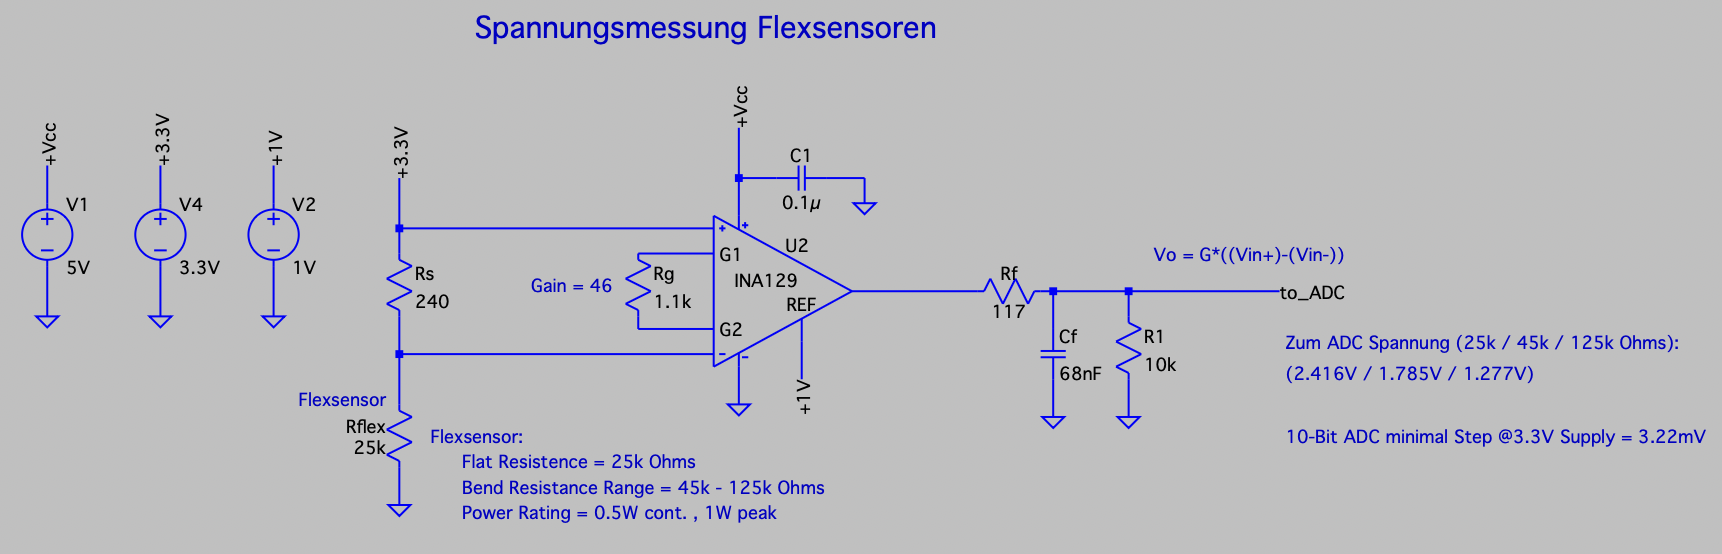
\includegraphics[width=0.8 \linewidth]{Simulation_Spannungsmessung_Flexsensoren}}
		%\caption*{Ladislaus Szabo}
	\end{center}
\end{figure}
\\
Die Flexsensoren (Rflex) beziehen ihre Versorgung über einen Shunt-Widerstand (Rs). Je nach Belastung, ändert sich der 
Spannungsabfall an diesem (Je größer die Beugung des Sensors, desto kleiner ist der Spannungsabfall). Die Spannungsdifferenz 
am Shunt-Widerstand wird von einem Operationsverstärker verstärkt. Bei der Auswahl des OPVs sind einige Punkte zu beachten, um 
eine korrerkte und genaue Erfassung der Fingerbeugung zu gewährleisten. \\
\\
Folgende Kriterien müssen folglich bei der Wahl des Operationsverstärkers beachtet werden:
\begin{itemize}
	\item Ausgangspegel bei gewählter Versorgungsspannung: \\
		  \\
		  Zunächst wurde das Kriterium der Versorgungsspannung betrachtet. Da wir maximal 5V Gleichspannung in der gesamten 
		  Schaltung verwenden wollen, muss der OPV mit dieser geringen Spannung immer noch verstärken. Da am positiven 
		  Verstärkereingang eine maximale Spannung von 3.3V anliegt, muss dies bei Verstärkern mit einer geeigneten Supply Range 
		  auch mit nur 5V Versorgungsspannung gewährleistet sein.
	\item Referenzspannung: \\
		  \\
		  Ein weiteres Kriterium ist das vorhanden sein eines Referenzspannungsanschlusses. Da der OPV keine Rail-to-Rail 
		  Technologie besitzt, muss der Ausgangsspannungspegel auf ein gewisses minimum angehoben werden. In unserem ist dies 
		  +1V. Würde diese Refernzspannung nicht vorhanden sein, so würde der OPV falsche Werte erzeugen, da dieser erst ab einer
		  verstärkten Spannung am Ausgang von ca. 750mV korrekt funktioniert.

\end{itemize}
Aufgrund dieser Kriterien und der Notwendigkeit von Genauigkeit und geringer Störungseigenschaften, viel die Wahl des 
Operationsverstärkers auf den INA129 instrumentation amplifier. \\
\\
Der Shunt-Widerstand wurde nicht berechnet. Dieser wurde einfach durch probieren inder Simulation bestimmt. \\
\\
Ein Tiefpassfilter (Rf und Cf) ist hinter den Ausgang des OPVs geschaltet, um mögliche Spannungsstörungen (Ripple), zusätzlich
zu dem ohnehin schon sehr störungsarmen Ausgangssignal des INA129, herauszufiltern. Der zu GND geschaltete Widerstand (R1), 
entlastet den Eingang des folgenden ADCs. Der Tiefpassfilter wurde folgendermaßen dimensioniert. \\
\\
\textbf{Berechnung des Tiefpassfilters:} \\
\\
\hspace*{1cm} $f_{g} = 20 kHz $ \hspace*{1cm} $\tau = \frac{1}{\omega_{g}} = \frac{1}{2\pi * 20 kHz} $ \\
\\
\hspace*{1cm} $f_{g} = \frac{\omega_{g}}{2\pi} $ \hspace*{1.7cm} $\tau = R * C $ \\
\\
\hspace*{4.25cm} $ C = 68 nF $ \hspace*{1cm} $ R = \frac{\tau}{68nF} = 117 \Omega $ \\
\\
\textbf{Berechnung der OPV Verstärkung und Dimensionierung des Shuntwiderstands:} \\
\\
\hspace*{1cm} Verstärkungsgleichung laut Datenblatt: $ G = 1+\frac{49.4k\Omega}{R_{g}} $ \\
\textcolor{red}{diemensionierung shuntwiderstand noch einfügen}
\\
\hspace*{1cm} Gain gewählt mit 46. \hspace*{1cm} $ R_{g} = 1.1k\Omega $ \\
\\
Die Verstärkung wurde so gewählt, dass diese mit dem Shunt-Widerstand für den ADC optimal geeignet ist. (Simulation) \\
\\
Der Shuntwiderstand wurde nicht wirklich berechnet. Dieser wurde durch probieren in der Simulation ermittelt. Eine Berechnung
des Shunts wäre nicht wirklich Zielführend gewesen, da diese normalerweise bei Schaltungen mit hohen Strömen verwendet werden. 
Da sich die Flexsensoren allerdings in einem Widerstandsbereich von $25k\Omega$ - $125k\Omega$ befinden, benötigen diese nicht
viel Strom, wodurch schon zu erwarten war, dass ein relativ hoher Wert benötigt wird. Schlussendlich wurden $240\Omega$ gewählt,
da dieser Widerstand bei sowohl voller, als auch geringer Biegung der Flexsensoren, eine gute Spannungsdifferenz für die 
Verstärkung mit dem OPV liefert. \\
\\
\textbf{Umwandlung der Differenzwerte in ein geeignetes Format:}
\\
Um nun die analogen Ausgangswerte des Operationsverstärkers nach der Verstärkung der Spannungsdifferenzen am Flexsensor für
den Mikrokontroller möglichst effizient und brauchbar zu machen, ist eine Umwandlung in ein digitales Signal notwendig.
Dies Funktion wird mit mit einem ADC umgesetzt. Bei der Wahl dieses Logikbauteils, sind, wie beim OPV, einige Kriterien zu 
beachten um die korrekte Funktion der Schaltung weiterhin zu gewährleisten. \\
\\
Folgende drei Kriterien sind maßgeblich bei der Wahl der Analog-Digital-Wandlers zu beachten:
\begin{itemize}
	\item Genauigkeit, Auflösungund Aussteuerbereich: \\
		  \\
		  \hspace*{1cm} $ Aussteuerbereich = 0 - 3.3V $ \\
		  \\
		  \hspace*{1cm} bei 10Bit ADC: $ LSB = 3.22mV $ \\
		  \\
		  \hspace*{1cm} Wegen der 1V Referenzspannung des OPVs ist der Ausgangspegel 1V - 3.3V \\
		  \\
		  \hspace*{1cm} $ ADC Ausgangsstufen = \frac{2.3V}{3.22mV} = 713 $ \\
\end{itemize}
Der reale Ausgangspegel des OPVs liegt wie bei der Simulation in Punkt Auslesen der Sensoren ermittelt zwischen 1.277V bis 2.416V.
Das beudeutet, dass eine Auflösung von 10Bit und ein Austeuerbereich von 0V - 3.3V ausreichend ist, um den kompletten Wertebereich
sehr genau abzudecken. Zusätzlich haben wir uns noch dazu entschieden alle Logikbauteile die eine Kommunikation mit dem Mikrokontroller
erfordern mit dem I2C Bussystem anzuschließen. Daher muss der Analog-Digital-Wandler diese Art der Kommunikation ebenfalls unterstützen.
Aufgrund dieser Auswahlkriterien ist die Wahl des Bauteils auf den MAX11611 gefallen.\\
\\
\textbf{Vervielfachung der Schaltung für alle Flexsensoren:}
\\
Um die zuvor beschriebene Schaltung nun nicht für jeden Flexsensor einzeln bauen zu müssen, wäre eine Art Schalter vorteilhaft.
Dieser soll in Sekundenbruchteilen zwischen allen Sensoren durchschalten. Das bedeutet also, dass zwischen dem Shunt-Widerstand
und $R_{flex}$ in der Simulation dieses Bauteil platziert werden muss. \\
\\
Für diesen Zweck ist ein Multiplexer bestens geeignet. Folgende Kriterien muss dieser erfüllen.
\begin{itemize}
	\item Versorgung und Kanäle: \\
		  \\ 
		  Die Versorgung muss an den Rest der Schaltung angepasst sein, das bedeutet, dass entweder 3.3V oder 5V in Frage kommen.
		  Bei einer Anzahl von einem Flexsensor pro Finger, also fünf, muss der Multiplexer mindestens 5 Kanäle aufweisen, wobei 
		  mehr Kanäle für mögliche zukünftige Erweiterungen kein Problem sind. All diese Eingänge müssen auf einen Ausgang geschalten
		  werden.
	\item Ansteuerung: \\
		  \\ 
		  Die Ansteuerung muss mit einem Mikrokontroller möglich sein. Hier bleibt also die Wahl zwischen analogen und digitalen 
		  Anschlüssen, oder ein I2C Anschluss um mit dem Rest der Schaltung kompatibel zu bleiben.
\end{itemize}
Folglich viel die Wahl auf den MUX508IDR. Dieser ist ein 8:1 Channel Multiplexer, der über 5V versorgt werden kann und über drei 
Analoganschlüsse für die Auswahl des Kanals verfügt. \\
\\
\textbf{Bewegungserfassung der Handgelenksdrehung:}
\\
Um die Drehung des Handgelenks zu erfassen ist ein anderer Sensor als ein Flexsensor notwendig. Dieser neue Sensor muss die 
Funktion eines Gyroskops haben und folglich die Positionen von X, Y -und Z-Achse übermitteln. Dieser Übermittlung muss per
I2C-Bus erfolgen, um die Kompatiblität mit der restlichen Schaltung zu ermöglichen. \\
\\
Ausgewählt wurder der Sensor MPU-6000, da dieser schon eingebaute ADCs hat, um die Achswerte vor der Übertragung zu digitalisieren. \\
\\
\textbf{Mikrokontroller:}
\\
Bei der Auswahl des Mikrokontrollers wurden sehr viele Aspekte beachtet. Dieser ist das Herzstück der Schaltung und ermöglicht
allen Komponenten zusammen zu funktionieren und diese auch zu steuern. \\
\\
Folgende Kriterien müssen vonn dem verwendeten Mikrokontroller folglich erfüllt werden:
\begin{itemize}
	\item Performancerelevante Ressourcen: \\
		  \\
		  Zu beachten ist hierbei vor allem der vorhandene Flash-Speicher, die CPU und der On-Chip Memory. Hierbei gilt grundsätzlich 
		  natürlich je mehr, desto besser. Das gleiche gilt ebenfalls für den Flash-Speicher.
	\item Versorgung und Anschlüsse: \\
		  \\
		  Um mit der Schaltung kompatibel zu sein, muss der Mikrokontroller mit 3.3V oder 5V versorgt werden können. Zusätzlich
		  sollte der Chip möglichst wenig Leistung brauchen. Es sollten mindestens zehn I/O-Anschlüsse vorhanden sein.
	\item Unterstützte Bussysteme: \\
		  \\
		  Da die wir bei der Schaltung eunheitlich auf das I2C Bussystem setzen, muss zumindest dieses von dem gewählten Mikrokontroller
		  unterstützzt werden. Als zweite Pflichtunterstützung gilt die UART-Kommunikation. Die Funktion und Notwendigkeit dieser
		  wird in Punkt \textcolor{red}{(externe Anschlüsse)} erläutert.
	\item Möglichkeiten der drahtlosen Übertragung: \\
		  \\
		  Da die Flexsensorwerte drahtlos Übertragen werden müssen, muss der Mikrokontroller eine Form dieser Übertragung unterstützen.
		  Vorzüglicherweise ist die Antenne für die Übertragung schon vorhanden, damit weitere Schaltungsteile nicht notwendig sind.
		  Hier kämen zum Beispiel Bluetooth oder Wifi in Frage.
	\item Programmierbarkeit: \\
		  \\
		  Der Chip muss mit einer schon verfügbaren Entwicklungsumgebung programmierbar sein. Wichtig ist in diesem Bezug vor allem
		  die Debugmöglichkeit, da bei einigen Mikrokontrollern ein extra Debugtool um viel Geld erworben werden muss. Eine Programmierung
		  im Terminal kommt ebenfalls nicht in Frage.
	\item Größe und Formfaktor: \\
		  \\
		  Schlussendlich dürfen sich alle Kriterien jedoch nicht zu sehr auf die Größe des Mikrokontrollers auswirken. Diese sollte
		  natürlich so klein wie möglich sein und trotzdem Bauteile wie eine Antenne aufweisen.
\end{itemize}
Nach beachtung aller Kriterien haben wir uns für einen ESP32 Mikrokontroller entschieden. Hierbei blieb allerdings die Wahl zwischen
dem reinen Chip und dem Modul, bei dem die Antenne und andere Funktionalitäten, die andernfalls selbst gebaut werden müssten,
schon integriert sind. Nach Abwägungen von Größe und Performance, haben wir uns für das ESP32-WROOM-32E-N16 Modul entschieden.
Dieses hat eine integrierte Antenne, reichlich Performance und viel Flash-Speicher. Der Formfaktor ist bei allen diesen 
Funktionalitäten immer noch im Rahmen. \\
\\
\textbf{Akkuversorgung:}
\\
Da es nicht praktikabel ist die Schaltung des Handschuhs dauerhaft mit einem Kabel zu versorgen, soll dies schlussendlich durch
einen Akku oder eine Batterie erfolgen. Entschieden haben wir uns für eine Lithium-Polymer-Akku (LiPo), da diese trotz geringer 
größe verglichen mit anderen Akkuarten eine hohe Kapazität besitzen. \\
\\
Die notwendige Kapazität für eine bestimmte Betriebsdauer wurde folgendermaßen berechnet:
\textcolor{red}{Berechnung Akkukapazität hier einfügen}
\\
Um den LiPo-Akku nicht jedes mal extern aufladen zu müssen, haben wir uns eine Schaltung überlegt, die dies auch mithilfe des
schon vorhandenen USB-C Anschlusses für das Programmieren des Mikrokontrollers verwendet wird. Dazu ist allerdings eine relativ 
komplitzierte Schaltung notwendig, weswegen bei vielen Produkten, die LiPo-Akkus verwenden, extra Ladegeräte gekauft werden müssen.
Dies wollten wir vermeiden und haben dementsprechend viel Zeit in die Reserche für eine funktionierende LiPo-Kontroller-Schaltung
investiert. \\
\\
Zunächst ist jedoch wichtig zu wissen, welchen Akku wir überhaupt erwenden. Entschieden haben wir uns für den \textcolor{red}{LiPo-Akku}.
\\

\subsubsection{Versuchsaufbauten und Messungen \textcolor{red}{Laci}}


\subsubsection{Schaltungsdesign \textcolor{red}{Laci}}
Nach den generellen Überlegungen, die zu der Entwicklung der Schaltung des Hanschuhs beigetragen haben, wird in diesem Punkt 
das genaue Schaltungsdesign erläutert. \\
\\
\textbf{Externe Anschlüsse:}
\begin{itemize}
	\item Anschluss zur Programmierung des Mikrokontrollers: \\
		  \\
		  Für die Programmierung des Mikrokontrollers wird ein USB Anschluss benötigt. Dieser sollte möglichst kompatibel mit
		  den neuesten Computern sein, weswegen wir uns für USB-C-Typ2.0 entschieden haben. Um das Serial Signal der USB Schnittstelle
		  für den Mikrokontroller lesbar zu machen, muss dieses für die UART-Kommunikation umgewandelt werden. Hierzu muss der Mikrokontroller
		  diese auch unterstützen. Mit einer Serial-UART-Bridge, wird das Signal umgewandelt. Der Chip wird von +3.3V versorgt.
		  Von der USB-Buchse werden die beiden Datenleitungen D+ und D- mit verbunden. Anschließend wird das umgewandelte Signal 
		  über die UART-Leitungen an den ESP32 Mikrokontroller übertragen. Wichtig zu beachten ist hierbei, dass die UART-Leitungen
		  ausgekreuzt sein müssen. Die Funktion der Anschlüsse RTS und DTR wird in Punkt \textcolor{red}{Mikrokontroller} erläutert. \\
		  \begin{figure}[H]
			\begin{center}
				\scalebox{0.5}
				{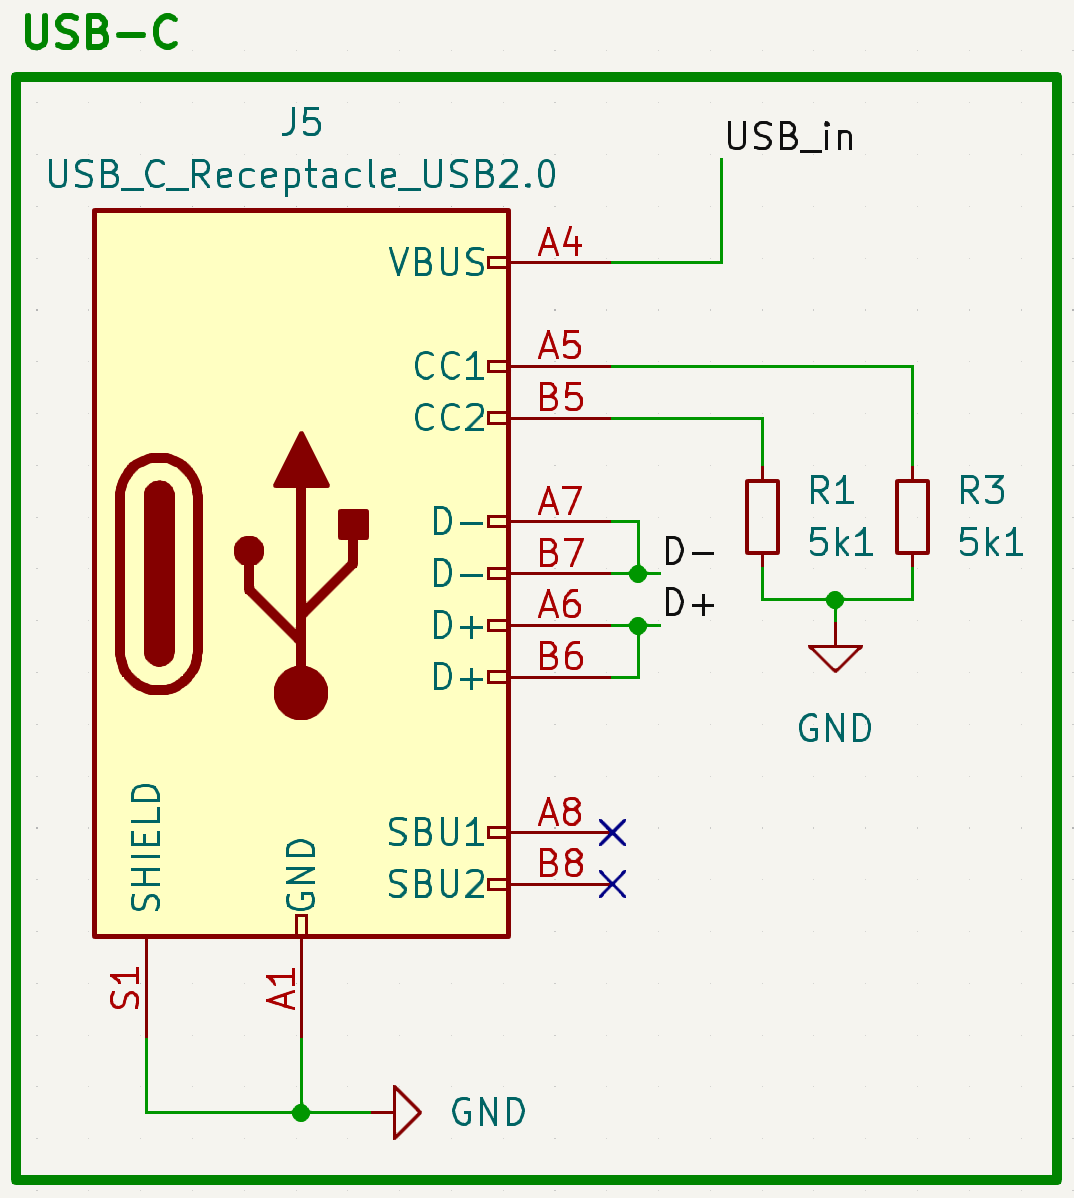
\includegraphics[width=0.8 \linewidth]{USB_C_Schaltplan_Handschuh}}
				%\caption*{Ladislaus Szabo}
			\end{center}
		\end{figure}
	\item Anschluss der Flexsensoren: \\
		  \\
		  Die Flexsensoren könnten natürlich einfach angelötet werden, jedoch ist die einfache Wartung bei einem fehlerhaften
		  Sensor ebenfalls zu berücksichtigen. Aufgrund dessen wird eine 6-Pin-JST-Buchse als Anschluss verwendet. Alle GND-Pins
		  werden auf einen zusammengefasst, um möglichst viel Platz zu Sparen. \\
		  \begin{figure}[H]
			\begin{center}
				\scalebox{0.5}
				{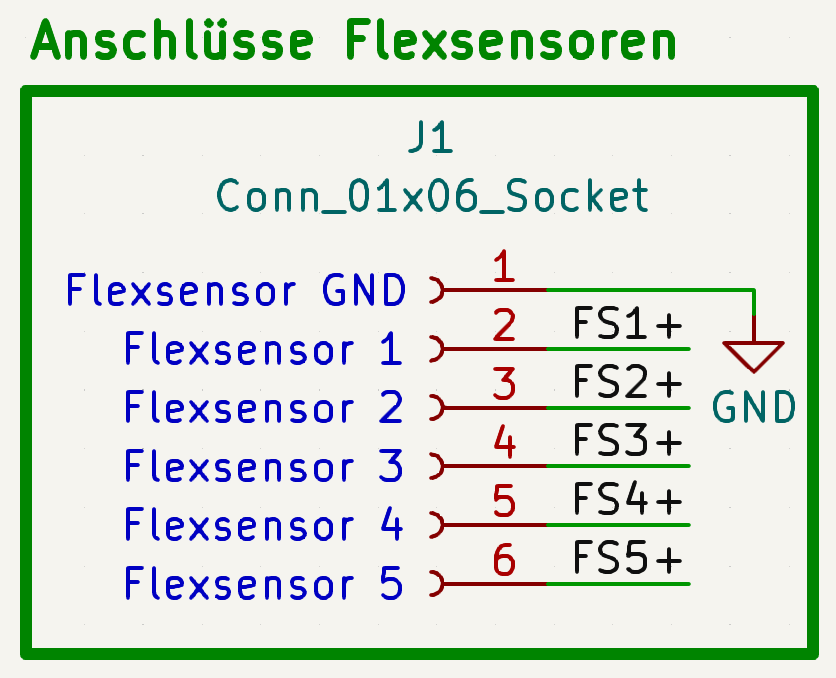
\includegraphics[width=0.8 \linewidth]{JST_Flexsensoren_Schaltplan_Handschuh}}
				%\caption*{Ladislaus Szabo}
			\end{center}
		\end{figure}
	\item Anschluss des Akkus: \\
		  \\
		  Der Akku wird ebenfalls mit einer JST-Buchse mit der Schaltung verbunden anstatt diesen anzulöten. Da der Akku einen
		  Versorgungs -und GND-Anschluss hat, wird eine 2-Pin-JST-Buchse verwendet. \\
		  \begin{figure}[H]
			\begin{center}
				\scalebox{0.5}
				{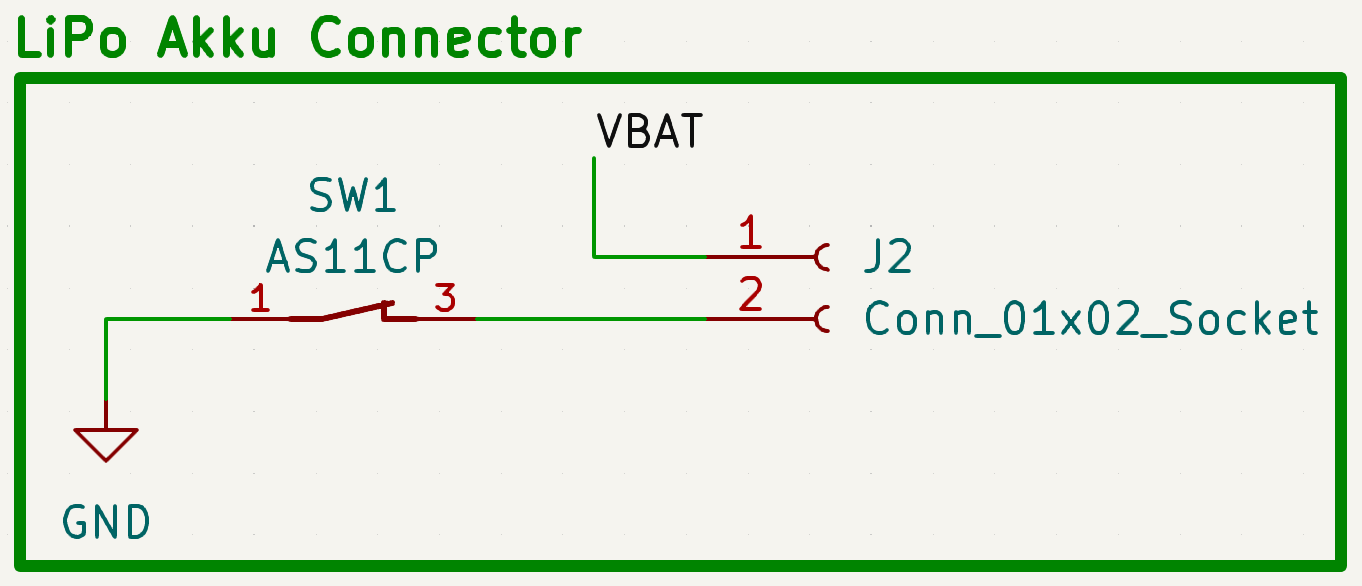
\includegraphics[width=0.8 \linewidth]{JST_Akku_Schaltplan_Handschuh}}
				%\caption*{Ladislaus Szabo}
			\end{center}
		\end{figure}\end{itemize}

\textbf{Mikrokontroller:} 
\\
Der ESP32-Chip wird mit +3.3V versorgt. Wichtig zu beachten ist dadurch, das ein Logic-HIGH somit auch 3.3V und nicht 5V ist!
Die Versorgung wird mit einem Kondensator stabilisiert. Für alle Busleitungen, also I2C und UART, wurden Widerstände in Serie
hinzugefügt, um die Kommunikationsleitungen vor Spannungsspitzen oder Überspannung zu schützen. Die Funktion wäre auch ohne diese
gegeben. Für die Datenleitungen SDA und SCL des I2c Busses sind zwei $10k\Omega$ PullUp-Widerstände vorgesehen. Zusätzlich 
wird ebenfalls der Anschluss IO16 mit einem PullUp-Widerstand auf 3.3V gezogen, da dies so vom Datenblatt vorgegeben wird. 
Die Funktionen der einzelnen Anschlüsse werden in den folgenden Punkten gemeinsam mit den damit verbundenen Bauteilen näher erläutert. \\
\begin{figure}[H]
	\begin{center}
		\scalebox{0.5}
		{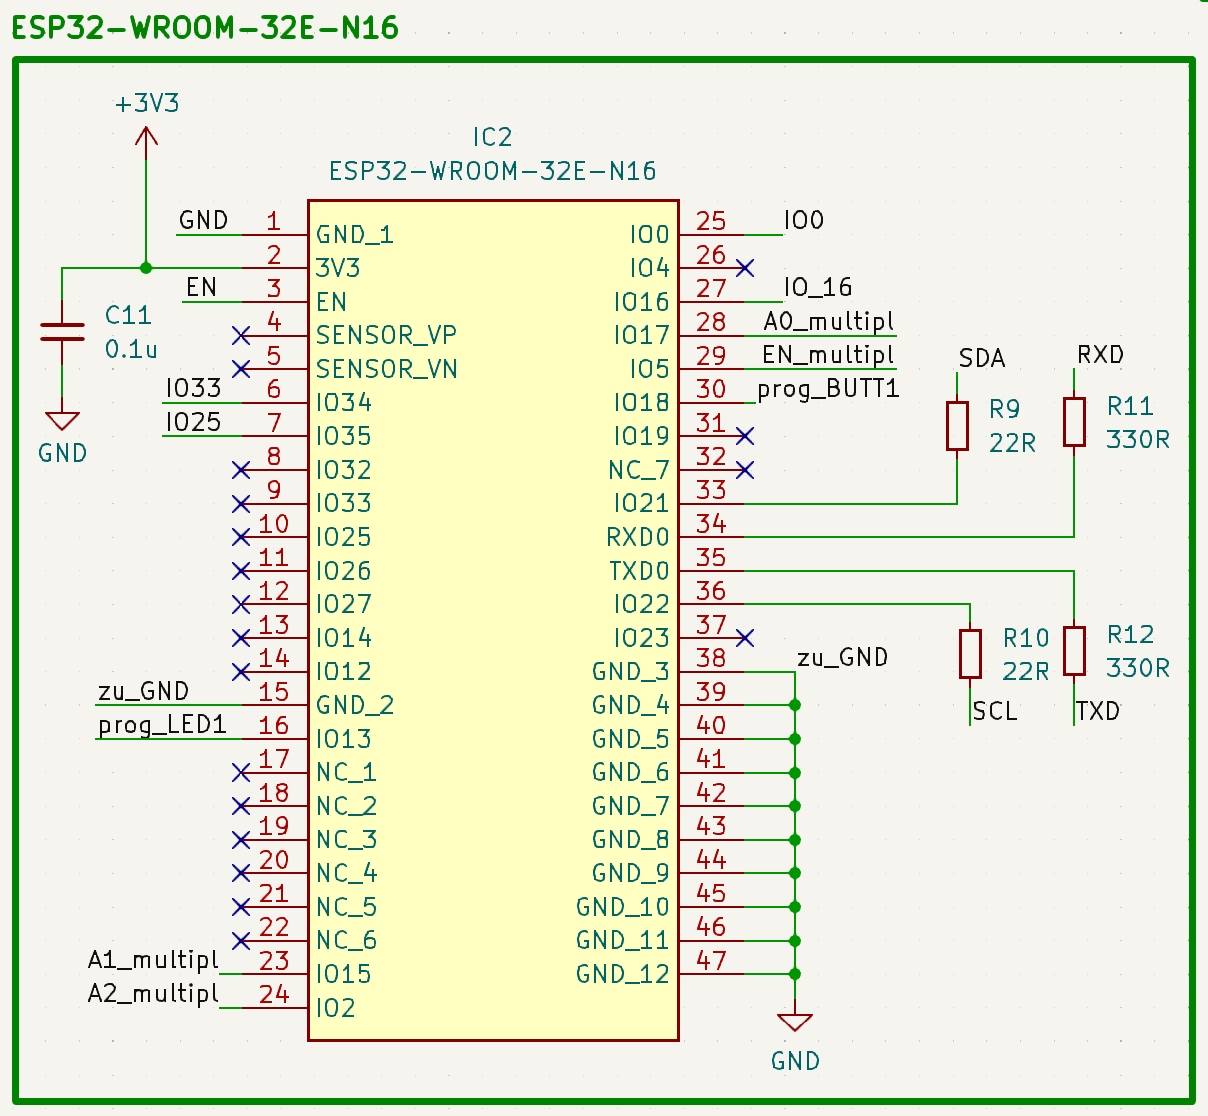
\includegraphics[width=0.8 \linewidth]{ESP32_Schaltplan_Handschuh}}
		%\caption*{Ladislaus Szabo}
	\end{center}
\end{figure}
\\
\textbf{Mikrokontroller Buttons:}
\\
In der Schaltung sind drei Taster verbaut. Diese sind alle mit dem Mikrokontroller verbunden und erfüllen verschiedene Funktionen.
\begin{itemize}
	\item Upload Button: \\
		  \\ 
		  Dieser Button ist mit dem IO0 Anschluss des ESP32 verbunden und muss bei dem Hochladen von Code kurzzeitig gedrückt 
		  werden, um den Mikrokontroller in den Upload-Modus zu versetzen. Der Pin IO0 ist standardmäßig für diese Funktion vorgesehen
		  und sollte für nichts anderes verwendet werden. 
	\item Reset Button: \\
		  \\
		  Dieser Button ist mit dem EN (Enable) Anschluss des ESP32 verbunden. Die Funktion dieses Tasters ist es, den ESP32 jederzeit 
		  zurücksetzen zu können falls dieser abstürtzt oder ein anderweitiges Problem auftritt, durch das dieser nicht mehr korrekt
		  funktioniert.
	\item Progrmmable Button: \\
		  \\
		  Die Funktion dieses Buttons kann frei durch den programmierten Code gewählt werden. 
\end{itemize}

\textbf{Status LEDs:}
\\
Die beiden Leuchtdioden sind als Statusanzeige gedacht. Eine POWER LED, die immer leuchtet wenn die Schaltung mit +5V
versorgt wird. Die Funktion der anderen LED ist, sowie bei einem Button, frei wählbar und ist deswegen mit Pin IO13 des ESP32
verbunden. \\
\begin{figure}[H]
	\begin{center}
		\scalebox{0.5}
		{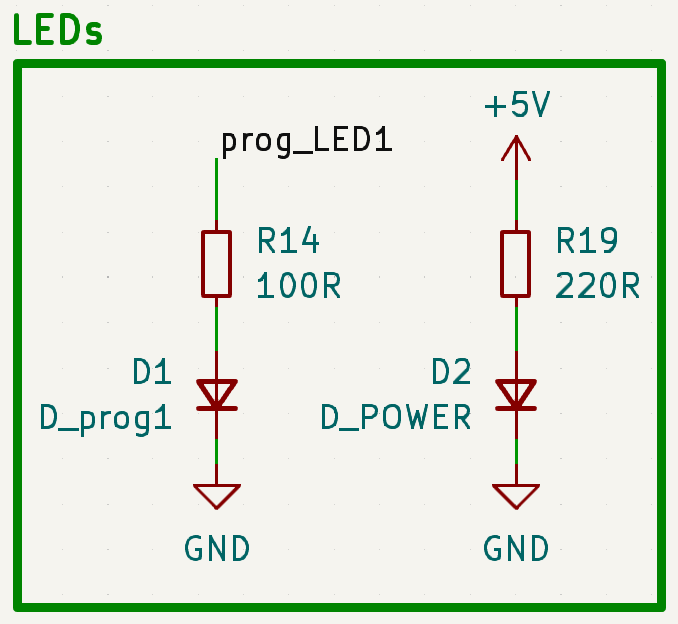
\includegraphics[width=0.8 \linewidth]{LEDs_Schaltplan_Handschuh}}
		%\caption*{Ladislaus Szabo}
	\end{center}
\end{figure}
\\
\textbf{Akku Versorgung:}
\\ 
\textbf{Multiplexer:}
\\
Der Multiplexer schaltet zwischen allen Flexsensoren durch und vermeidet somit die Messschaltung fünf mal bauen zu müssen. 
Die Verbindung zum ESP32 erfolgt über drei digitale Addresspins und einen Enable Pin. Je nachdem welche Bitkombination übermittelt
wird, ändert sich die interne Schalterposition und somit der gerade aktive Kanal zur Messung eines Flexsensors. \\
\\
\textbf{Operationsverstärker:}
\\
Für das Auslesen der Flexsensoren, wird eine Schaltung, wie in Punkt "Auslesen der Sensoren" beschrieben, benötigt. Da am
Shuntwiderstand nur sehr wenig Spannungsabfall auftritt und daher die Spannungsdifferenz zwischen positivem und negativem 
Verstärkereingang sehr klein ist, muss das Signal verstärkt werden. Hierfür wird der INA129 Instrumentenverstärker verwendet.
Dieser wird mit 5V versorgt, was für einen OPV eine relativ geringe Versorgungsspannung ist. Da die maximale Eingangsspannung
der Verstärkereingänge allerdings nie mehr als 3.3V beträgt, ist dies kein Problem. \\
\\
Die +1V Spannungsreferenz ist notwendig, da der ausgewählte Operationsverstärker nicht über Rail-to-Rail Technologie besitzt. 
Die kleinstmögliche Spannungsdifferenz am Eingang des OPV, wenn der Flexsensor seinen maximalen Widerstand von
$125k\Omega$ erreicht, beträgt nur 6.3mV. Aufgrund der fehlenden Rail-to-Rail Fähigkeit, muss die Ausgangsspannung des OPV deshalb
auf mindestens 800mV angehoben werden, um eine korrekte Funktion des OPVs zu gewährleisten. Deshalb wird eine Referenzspannung
von 1V verwendet. \\
\begin{figure}[H]
	\begin{center}
		\scalebox{0.5}
		{\includegraphics[width=0.8 \linewidth]{Operationsverstärker_Schaltplan_Handschuh}}
		%\caption*{Ladislaus Szabo}
	\end{center}
\end{figure}
\\
\textbf{Analog-Digital-Wandler:}
\\
\begin{figure}[H]
	\begin{center}
		\scalebox{0.5}
		{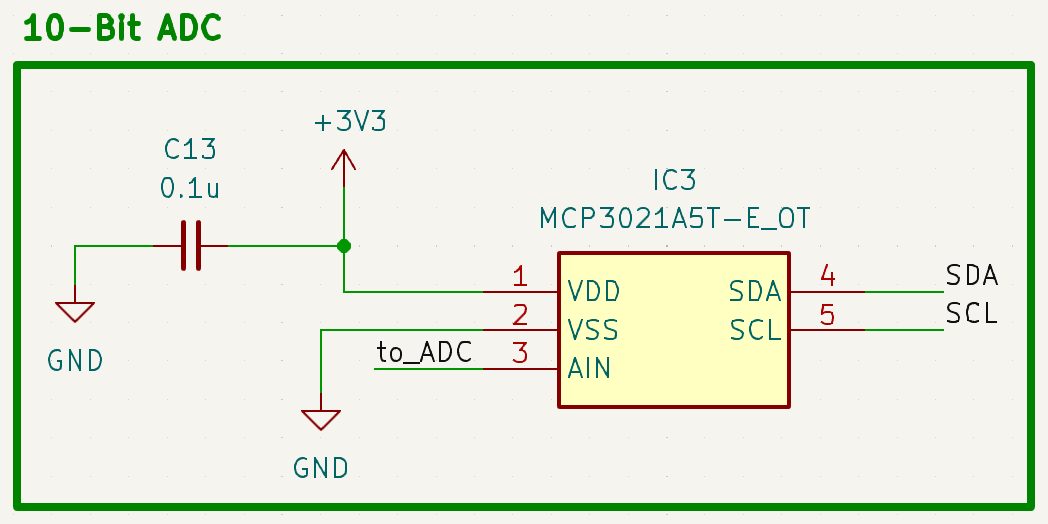
\includegraphics[width=0.8 \linewidth]{ADC_Schaltplan_Handschuh}}
		%\caption*{Ladislaus Szabo}
	\end{center}
\end{figure}
\\
\textbf{Gyroskop-Sensor:}
\\
\begin{figure}[H]
	\begin{center}
		\scalebox{0.5}
		{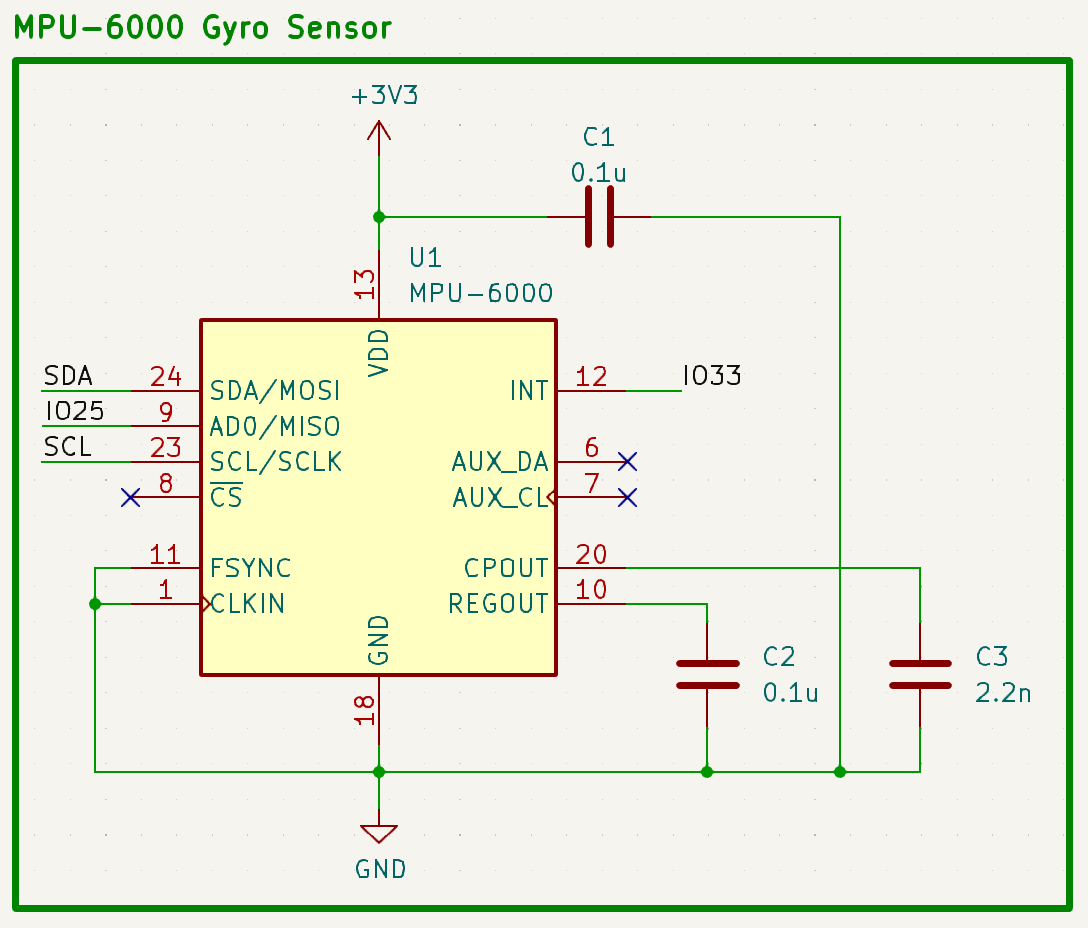
\includegraphics[width=0.8 \linewidth]{Gyro_Schaltplan_Handschuh}}
		%\caption*{Ladislaus Szabo}
	\end{center}
\end{figure}
\\
\textbf{Akku Versorgung:}
\\
\begin{figure}[H]
	\begin{center}
		\scalebox{0.5}
		{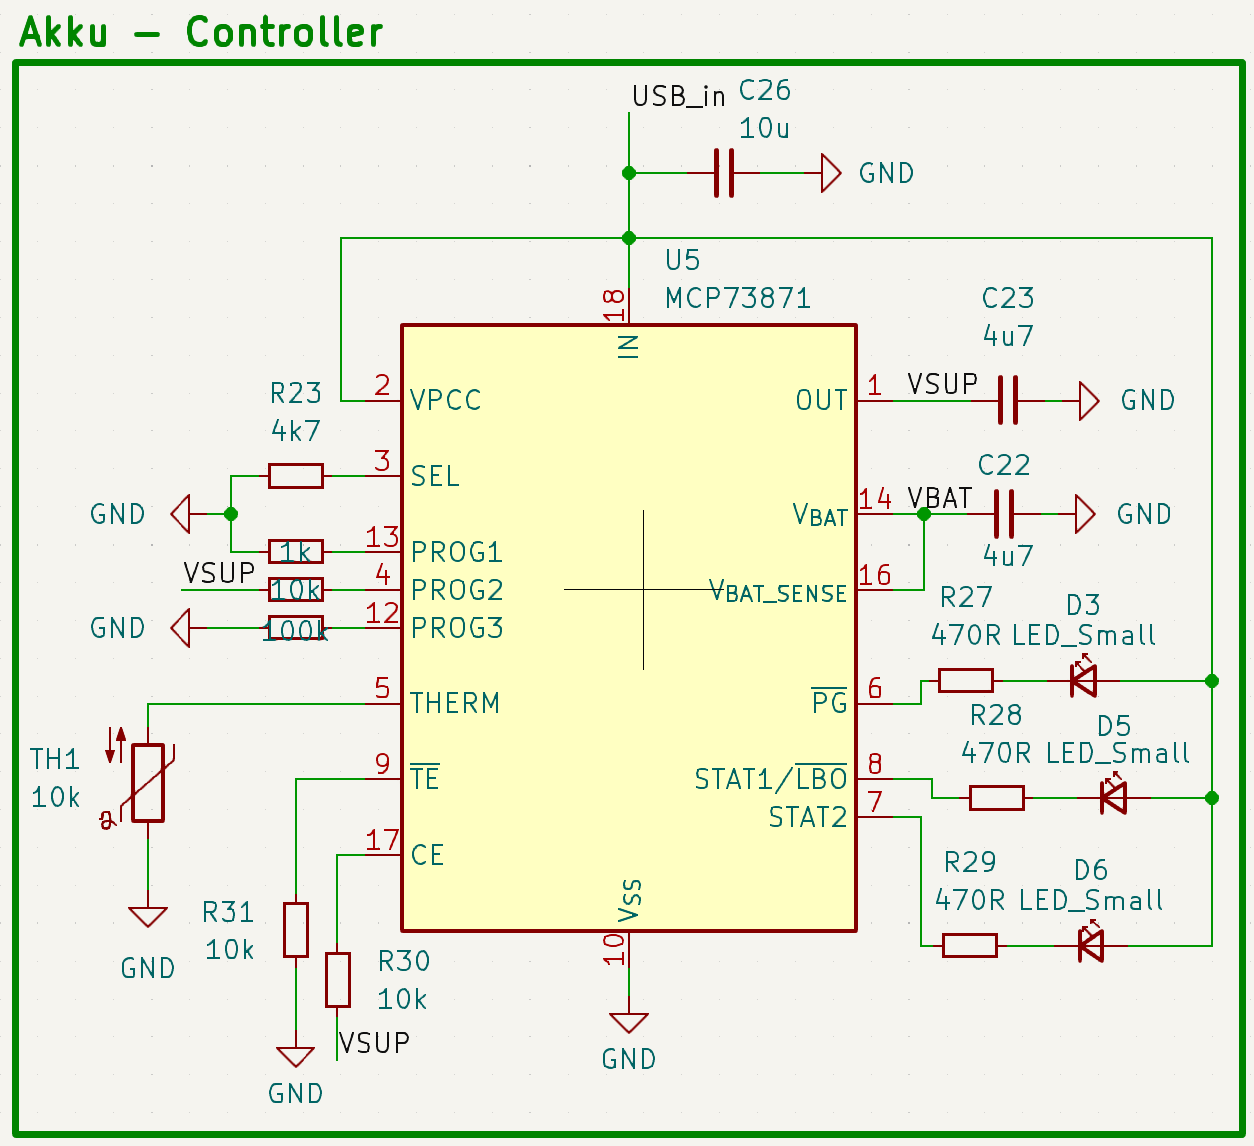
\includegraphics[width=0.8 \linewidth]{Akku_Controller_Schaltplan_Handschuh}}
		%\caption*{Ladislaus Szabo}
	\end{center}
\end{figure}
\\
\begin{figure}[H]
	\begin{center}
		\scalebox{0.5}
		{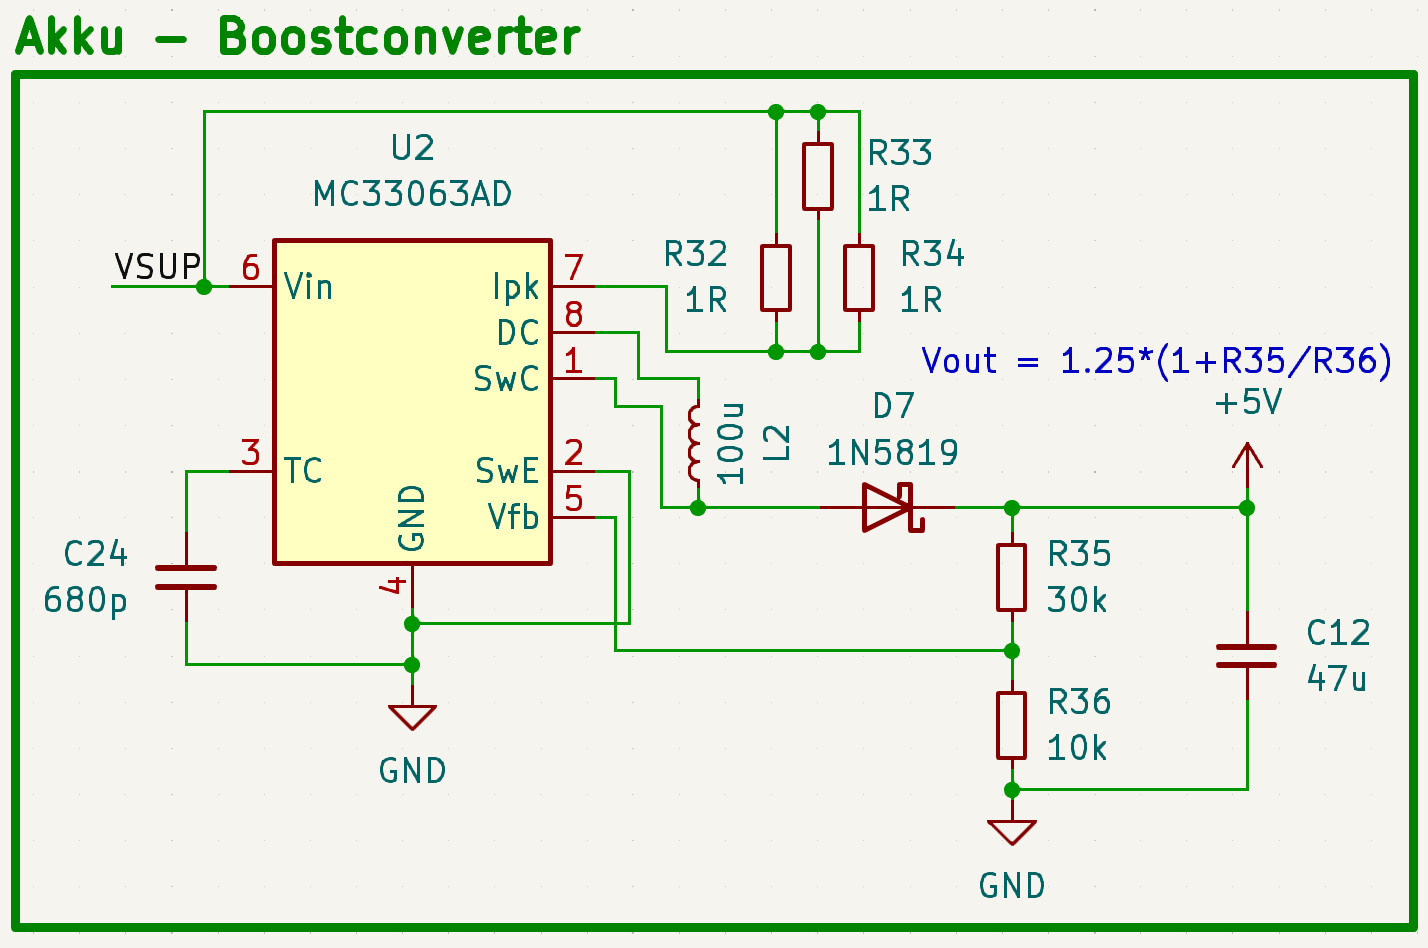
\includegraphics[width=0.8 \linewidth]{Akku_Boostconverter_Schaltplan_Handschuh}}
		%\caption*{Ladislaus Szabo}
	\end{center}
\end{figure}
\\
\begin{figure}[H]
	\begin{center}
		\scalebox{0.5}
		{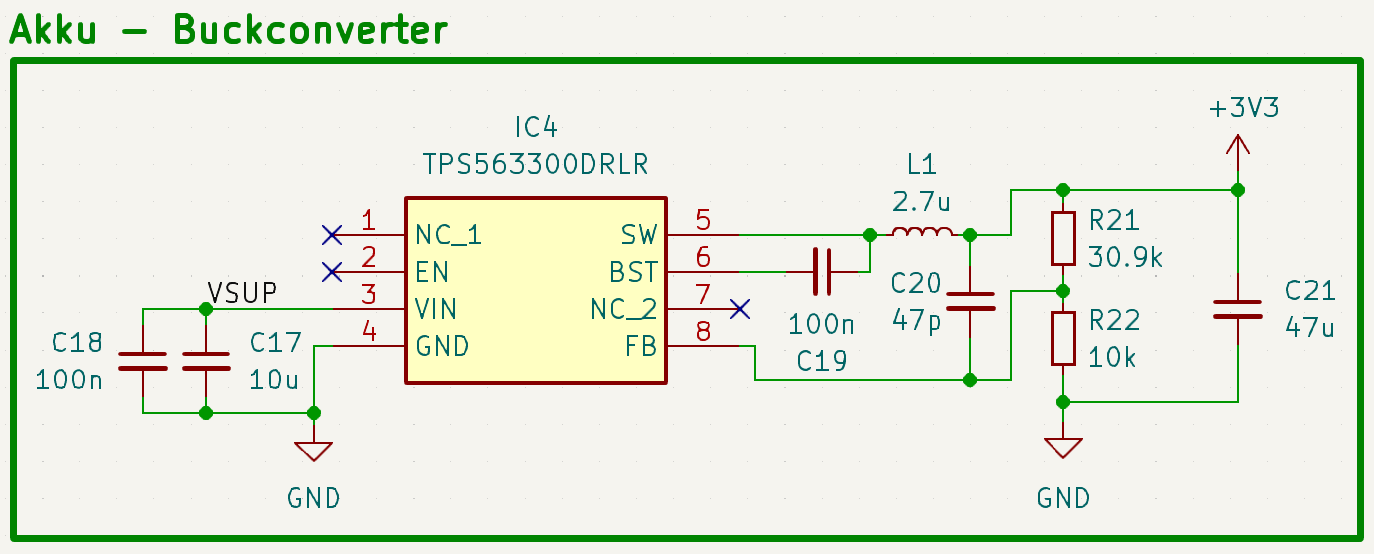
\includegraphics[width=0.8 \linewidth]{Akku_Buckconverter_Schaltplan_Handschuh}}
		%\caption*{Ladislaus Szabo}
	\end{center}
\end{figure}
\\
\subsubsection{Platinendesign \textcolor{red}{Laci}}

\subsection{Roboterhand}
\subsubsection{Simulationen und Versuchsaufbauten \textcolor{red}{Laci}}
\subsubsection{Überlegungen und Dimensionierung \textcolor{red}{Laci}}
\subsubsection{Schaltplandesign \textcolor{red}{Laci}}
\subsubsection{Platinendesign \textcolor{red}{Laci}}

%--------------------------------------------------------------------------
%--------------------------------------------------------------------------

\section{Softwareentwicklung}

\subsection{Handschuh}
\subsubsection{Konzepte und Überlegungen \textcolor{red}{Fabian}}
Datenübertragung:
Es gibt viele Möglichkeiten die Werte, die man von jedem einzelnen Flexsensor ausliest, zu übertragen. Wichtig ist es, dass 
dies einfach und auf eine sehr stabile Weise funktioniert. Anfangs war Bluetooth die favorisierte Option, später dann aber Wifi. 
Schlussendlich wurde es dann ESP-NOW, das auf 2,4GHz funkt und am ehesten mit Wifi verglichen werden kann. Es können pro 
Sendung 250 Byte gesendet werden. Ebenso ist eine Kommunikation zwischen mehreren ESP32 in beide Richtungen möglich. Der 
Standard gilt allerdings wirklich nur für den ESP32, was allerdings aufgrund der Wahl von nur diesen letztgenannten, keine 
Probleme darstellt.

\subsubsection{Realisierung und Gliederung \textcolor{red}{Fabian}}

\subsection{Roboterhand}
\subsubsection{Konzepte und Überlegungen \textcolor{red}{Fabian}}
\subsubsection{Realisierung und Gliederung \textcolor{red}{Fabian}}

\subsection{User Interface}
\subsubsection{Entwicklungsumgebung \textcolor{red}{Laci}}
\subsubsection{Konzepte und Überlegungen \textcolor{red}{Laci}}
\subsubsection{Realisierung und Gliederung \textcolor{red}{Laci}}

%--------------------------------------------------------------------------
%--------------------------------------------------------------------------

\section{Abschluss und Zusammenfassung}

%--------------------------------------------------------------------------
%--------------------------------------------------------------------------

\section{Anhang}
\section{Quellen -und Literaturverzeichnis}
\section{Abbildungsverzeichnis}

\end{document}